\documentclass[../main-sheet.tex]{subfiles}
\usepackage{../style}
\graphicspath{ {../img/} }
\backgroundsetup{contents={}}
\begin{document}
\chapter{Epidemic Models and Dynamics of Infectious Diseases}
\section{Epidemiology}
Epidemiology is the study of the distribution and determinants of disease frequency in human population (or in the group of population). It is the cornerstone of public health and informs policy decisions and evidence-based medicine by identifying risk factors for disease and targets for preventive medicine.
\section{Endemic}
Endemic is the habitual presence of a disease within a given geographic area.
\section{Epidemic}
The epidemic is the occurrence in a community or region of a group of illnesses of similar nature in excess of normal expectancy and distributed from a common or propagated source.
\section{Pandemic}
The pandemic is a worldwide epidemic.

There are various types of epidemiological models. We can classify them into two classes:
\begin{enumerate}[label=(\roman*)]
    \item disease with removal,
    \item disease without removal.
\end{enumerate}
\section{Epidemic models with removal}
The model considers the diseases which have the property that individuals once infected by these diseases will be removed from the disease through recovery or death. The individuals removed through recovery are immune temporarily or permanently.

In this case we have three classes of individuals.
\begin{enumerate}[label=(\roman*)]
    \item The susceptible class \((S)\)
    \item The infective class \((I)\)
    \item The removal class \((R)\)
\end{enumerate}
\section{Susceptible class}
The susceptible class consists of those individuals who are not infective but who are capable of catching the disease.
\section{Infective class}
The infective class consists of those individuals who are capable of transmitting the disease to others.
\section{Removal class}
The removal class consists of those individuals who had the disease are dead or recovered or permanently immune or isolated until recovery.
\begin{prob}
    Assume that \(t_0<t_1<t_2\) are equally spaced time values. Let the corresponding population size are \(P_0\), \(P_1\), \(P_2\) respectively. Then the growth rate \(a\) and the carrying capacity \(k\) of logistic population are
    \[
        a=\frac{1}{t_0-t_1}\ln \left[ \frac{\frac{1}{P_2}-\frac{1}{P_1}}{\frac{1}{P_1}-\frac{1}{P_0}} \right]
    \]
    \[
        K=\frac{\frac{2}{P_1}-\frac{1}{P_0}-\frac{1}{P_2}}{\frac{1}{P_1^2}-\frac{1}{P_0P_2}}
    \]
\end{prob}
\begin{soln}
    We have
    \begin{equation}
        P(t)=\frac{K}{1+\left( \frac{K}{P_0}-1 \right)e^{-a(t-t_0)}}
        \label{eq:defnprob1.1}
    \end{equation}
    \begin{align*}
        \Rightarrow\;\frac{1}{P(t)}&=\frac{1}{K}\left[ 1+\left( \frac{K}{P_0}-1 \right)e^{-a(t-t_0)} \right]\\
        &=\frac{1}{K}\left[ 1-e^{-a(t-t_0)} \right]+\frac{1}{P_0}e^{-a(t-t_0)}
    \end{align*}
    \begin{equation}
        \therefore\; \frac{1}{P_1}=\frac{1}{K}\left[ 1-e^{-a(t_1-t_0)} \right]+\frac{1}{P_0}e^{-a(t_1-t_0)}
        \label{eq:defnprob1.2}
    \end{equation}
    and
    \begin{equation}
        \therefore\; \frac{1}{P_2}=\frac{1}{K}\left[ 1-e^{-a(t_2-t_0)} \right]+\frac{1}{P_0}e^{-a(t_2-t_0)}
        \label{eq:defnprob1.3}
    \end{equation}
    Now \eqref{eq:defnprob1.3}-\eqref{eq:defnprob1.2}, we have
    \begin{align*}
        \frac{1}{P_2}-\frac{1}{P_1}&=\frac{1}{K}\left[ 1-e^{-a(t_2-t_0)}-1+e^{-a(t_1-t_0)} \right]+\frac{1}{P_0}e^{-a(t_2-t_0)}-\frac{1}{P_0}e^{-a(t_1-t_0)}\\
        &=\left( \frac{1}{P_1}-\frac{1}{P_0} \right)e^{-a(t_1-t_0)} \quad[\text{Since \(t_0<t_1<t_1\) are equally spaced. So \(t_1=t_2\), \(t_0=t_1\)}]
    \end{align*}
    \begin{equation}
        e^{-a(t_1-t_0)}=\frac{\frac{1}{P_2}-\frac{1}{P_1}}{\left( \frac{1}{P_1}-\frac{1}{P_0} \right)}
        \label{eq:defnprob1.4}
    \end{equation}
    \begin{align*}
        \Rightarrow\;\;& a(t_0-t_1)=\ln\left[ \frac{\frac{1}{P_2}-\frac{1}{P_1}}{\left( \frac{1}{P_1}-\frac{1}{P_0} \right)} \right]\\
        \therefore\;\;& a=\frac{1}{t_0-t_1}\ln\left[ \frac{\frac{1}{P_2}-\frac{1}{P_1}}{\left( \frac{1}{P_1}-\frac{1}{P_0} \right)} \right]
    \end{align*}
    From \eqref{eq:defnprob1.2} we have,
    \begin{align*}
        &\frac{1}{P_1}-\frac{1}{P_0}e^{-a(t_1-t_0)}=\frac{1}{K}\left[ 1-e^{-a(t_1-t_0)} \right]\\
        \Rightarrow\; &K=\frac{ 1-e^{-a(t_1-t_0)}}{\frac{1}{P_1}-\frac{1}{P_0}e^{-a(t_1-t_0)}}\\
        \Rightarrow\; &K=\frac{\displaystyle 1-\frac{\frac{1}{P_2}-\frac{1}{P_1}}{\frac{1}{P_1}-\frac{1}{P_0}} }{\displaystyle \frac{1}{P_1}-\frac{1}{P_0}\left( \frac{\frac{1}{P_2}-\frac{1}{P_1}}{\frac{1}{P_1}-\frac{1}{P_0}} \right)}\qquad [\text{Using \eqref{eq:defnprob1.4}}]\\
        \Rightarrow\; &K=\frac{\displaystyle \frac{\frac{1}{P_1}-\frac{1}{P_0}-\frac{1}{P_2}+\frac{1}{P_1}}{\frac{1}{P_1}-\frac{1}{P_0}}}{\displaystyle \frac{\frac{1}{P_1^2}-\frac{1}{P_0P_1}-\frac{1}{P_0P_2}+\frac{1}{P_0P_1}}{\frac{1}{P_1}-\frac{1}{P_0}}}\\
        \therefore\; &K=\frac{\displaystyle \frac{2}{P_2}-\frac{1}{P_0}+\frac{1}{P_2}}{\displaystyle \frac{1}{P_1^2}-\frac{1}{P_0P_2}}
    \end{align*}
\end{soln}
\begin{prob}
    What do you mean by disease with removal and without removal?
\end{prob}
\begin{soln}
    The epidemic logistic models are various in type such as
    \begin{enumerate}[label=(\roman*)]
        \item Disease without removal
        \item Disease with removal
    \end{enumerate}
    \emph{Disease without removal:} In this case, it is assumed that persons are infected can never be removed from the disease. Therefore, the total population always remains either in \(S\) class or in \(I\) class.

    \emph{Example}: \(SI\) and \(SIS\) models etc. are disease without removal model.\\

    \emph{Disease with removal:} In this model, we consider those diseases which are of the nature, individuals once infected can be removed from the disease through recovery or death. This removal may be temporary or permanent.

    \emph{Example:} Several types of this model are \(SIR\) model, \(SIRS\), \(SEIR\) etc.
\end{soln}
\begin{prob}
    Describe \(SIS\) model.
\end{prob}
\begin{soln}
    The \(SIS\) model is given by
    \begin{align}
        \ddt{S}&=-\alpha SI-\beta I \label{eq:si1}\\
        \ddt{I}&=\alpha SI-\beta I \label{eq:si2}
    \end{align}
    where, \(\begin{aligned}[t]
        S(t)&= \text{ the number of susceptible individuals at time } t\\
        I(t)&= \text{ the number of infected individuals at time } t
    \end{aligned}\)\\
    where \(\alpha\) and \(\beta\) are the constant and
    \begin{equation}
        S+I=N\label{eq:si3}
    \end{equation}
    where \(N\) is the size of the population.\\

    In this model we assume that a susceptible person becomes infected at a rate proportional to \(SI\) and then an infected person recovers and again becomes susceptible at rate proportional to \(I_0\).\\
    The above model has the initial condition, \(S(0)=S_0\), \(I(0)=I_0\) at \(t=0\).\\
    We have, \(S(t)+I(t)=S_0+I_0=\) constant \(=N\).\\
    From \eqref{eq:si2},
    \begin{align}
        &\ddt{I}=\alpha (N-I)I-\beta I\notag\\
        \Rightarrow\;&\ddt{I}=\alpha NI-\alpha I^2-\beta I\notag\\
        \Rightarrow\;&\ddt{I}=I(\alpha N-\beta)-\alpha I^2\notag\\
        \Rightarrow\;&\ddt{I}=K I-\alpha I^2\qquad \text{where, }K=\alpha N-\beta\notag\\
        \Rightarrow\;&\ddt{I}=KI\left( 1-\frac{\alpha}{K}I \right)\notag\\
        \Rightarrow\;&\frac{\D I}{I\left( 1-\frac{\alpha}{K}I \right)}=K\D t\notag\\
        \Rightarrow\;&\left[ \frac{1}{I}+\frac{1}{\frac{K}{\alpha}-I} \right]\D I=K\D t\notag\\
        \Rightarrow\;&\ln{I}+\ln\left[\frac{K}{\alpha}-I \right]=Kt+\ln A\notag\\
        \Rightarrow\;& \ln \frac{I}{A\left[ \frac{K}{\alpha}-I \right]}=Kt\notag\\
        \Rightarrow\;& \frac{I}{A\left[ \frac{K}{\alpha}-I \right]}=e^{Kt}\notag\\
        \Rightarrow\;& A=\frac{I}{\left[ \frac{K}{\alpha}-I \right]e^{Kt}}\label{eq:si4}\\
        \Rightarrow\;& A\frac{K}{\alpha}e^{Kt}-AIe^{kt}=I\notag\\
        \Rightarrow\;& I=\frac{A\frac{K}{\alpha}e^{Kt}}{1+Ae^{Kt}}\label{eq:si5}
    \end{align}
    Initially, \(t=0\), \(I=I_0\), \(A=\frac{I_0}{\frac{k}{\alpha}-I_0}\)\\
    From \eqref{eq:si5},
    \begin{align*}
        I&=\frac{I_0 \left[\frac{K}{\alpha}\right]e^{Kt}}{\left(\frac{k}{\alpha}-I_0\right) \left[1+\frac{I_0}{\frac{k}{\alpha}-I_0}\right]e^{Kt}}\\
        &=\frac{I_0 \frac{K}{\alpha}e^{Kt}}{\frac{k}{\alpha}-I_0+{I_0}e^{Kt}}\\
        &=\frac{\frac{K}{\alpha}I_0 e^{kt}}{I_0\frac{k}{\alpha}\left[ \frac{1}{I_0}+\left( e^{kt}-1 \right)\frac{\alpha}{k} \right]}\\
        &=\frac{e^{kt}}{\frac{\alpha}{k}\left( e^{kt}-1 \right)+\frac{1}{I_0}}\qquad \text{where }k\neq0
    \end{align*}
    When \(k=0\), 
    \begin{align*}
        &\ddt{I}=-\alpha I^2\\
        \Rightarrow\;&-\frac{\D I}{I^2}=\alpha \D t\\
        \Rightarrow\;&\frac{1}{I}=\alpha +B\\
        \intertext{Initially, \(t=0\), \(I=I_0\)}
        \therefore\;&B=\frac{1}{I_0}\\
        \therefore\;&\frac{1}{I}=\alpha +\frac{1}{I_0}\\
        \Rightarrow\;&I=\frac{1}{\alpha t+\frac{1}{I_0}}
    \end{align*}
    \[
        I(t)=\begin{cases}
        \frac{e^{kt}}{\frac{\alpha}{k}\left( e^{kt}-1 \right)+\frac{1}{I_0}},&k\neq 0\\
        \frac{1}{\alpha t+\frac{1}{I_0}},&k=0
        \end{cases}
    \]
    Since, \(S(t)+I(t)=N\), i.e., \(S(t)=N-I(t)\)\\
    We get,
    \[
        S(t)=\begin{cases}
        N-\frac{e^{kt}}{\frac{\alpha}{k}\left( e^{kt}-1 \right)+\frac{1}{I_0}},&k\neq 0\\
        N-\frac{1}{\alpha t+\frac{1}{I_0}},&k=0
        \end{cases}
    \]
    We have, \(k=\alpha N-\beta\quad\Rightarrow\;\frac{K}{\alpha}=N-\frac{\beta}{\alpha}=N-\rho\) where \(\rho=\frac{\beta}{\alpha}\) is known relative removal rate.\\
    Now, as \(\begin{aligned}[t]
        t&\to \infty,\\
        I(t)&\to \frac{k}{\alpha}=N-\rho\quad \text{if }k>0, \text{i.e., }N>\rho\\
        \text{and }I(t)&\to 0\quad \text{if }k\leq 0, \text{i.e., }N\leq\rho
    \end{aligned}\)\\

    These results are shown in the diagram.
    \begin{center}
        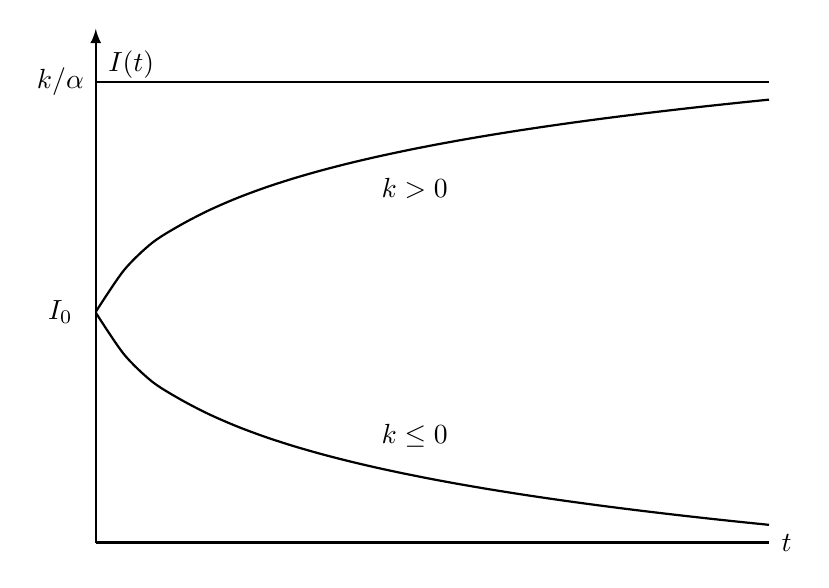
\begin{tikzpicture}[scale=.9]
            \draw[thick] (0.5,3.25)--(10,3.25);
            \draw[thick] (0.5,-3.25)--(10,-3.25);
            \draw[thick,-latex] (0.5,-3.25)--(.5,4);
            \draw [thick, smooth, domain=0.5:10] plot ({\x}, {ln(.1*\x)+3});
            \draw [thick, smooth, domain=0.5:10] plot ({\x}, {-(ln(.1*\x)+3)});
            
            \node at (10.25,-3.25) {$t$};
            \node at (0,0) {$I_0$};
            \node at (0,3.25) {$k/\alpha$};
            \node at (1,3.5) {$I(t)$};
            \node at (5,1.75) {$k>0$};
            \node at (5,-1.75) {$k\leq 0$};
            \end{tikzpicture}
    \end{center}
\end{soln}
\begin{prob}
    If the population of a country double in 50 years, in how many years will it triple under the assumption of the Malthusian model? What will be the population in the year 2000?
\end{prob}
\begin{soln}
    We have from Malthusian model,
    \begin{equation}
        N=N_0e^{K(t-t_0)}\label{eq:probdef2.1}
    \end{equation}
    Suppose at \(t-t_0=50\) years, the population will be double in size. i.e., \(N=2N_0\).\\
    From \eqref{eq:probdef2.1} 
    \begin{align*}
        &2N_0=N_0 e^{K\times 50}\\
        \Rightarrow\;\;& e^{50K}=2\\
        \Rightarrow\;\;& {50K}=\ln 2\\
        \Rightarrow\;\;& k=\frac{1}{50}\ln 2\\
        \therefore\;\;& k=0.01386
    \end{align*}
    For population to be tripled \(N=3N_0\), \(t-t_0=?\)\\
    From \eqref{eq:probdef2.1} 
    \begin{align*}
        &3N_0=N_0 e^{K(t-t_0)}\\
        \Rightarrow\;\;&3= e^{0.01386(t-t_0)}\\
        \Rightarrow\;\;& (t-t_0)=\frac{\ln 3}{0.01386}=79.26\text{ years}
    \end{align*}
    After 79.26 years, the population will be triple.
\end{soln}
\begin{prob}
    Use the logistic model with an assumed carrying capacity of \(100\times 10^9\) an observed population of \(5\times 10^9\) in 1986 and an observed rate of growth of \(2\%\) per year when population size is \(5 \times 10^9\) predict the population of the earth in the year 2008.
\end{prob}
\begin{soln}
    We have, from logistic model,
    \begin{equation}
        N(t)=\frac{K N_0}{N_0+(K-N_0)e^{-rt}}\label{eq:probdef3.1}
    \end{equation}
    Where, \(\begin{aligned}[t]
        k&=100\times 10^9\\
        r&=2\% = 0.02\\
        t&=2008-1968=22\\
        N_0&=5\times 10^9
    \end{aligned}\)\\

    Then from \eqref{eq:probdef3.1},
    \begin{align*}
        N(t)&=\frac{100\times 10^9\times 5\times10^9}{5\times 10^9+(100\times 10^9-5\times 10^9\times e^{-0.02\times 22})}\\
        &=\frac{500\times 10^{18}}{5\times 10^9+95\times 10^9\times e^{-0.44}}\\
        &=\frac{500\times 10^{18}}{10^9(5+95\times 0.6440)}\\
        &=7.55\times 10^9
    \end{align*}
\end{soln}
\begin{prob}
    The Pacific halibut fishery is modeled by the logistic equation with carrying capacity \(80.5\times 10^6\) measured in kilograms and intrinsic growth rate \(0.71\) per year. If the initial biomass is one fourth the carrying capacity find the biomass one year later and the time required for the biomass to grow to half the carrying capacity.
\end{prob}
\begin{soln}
    The logistic model is
    \begin{equation}
        x'=rx\left(1-\frac{x}{K}\right)\label{eq:probdef4.1}
    \end{equation}
    Given, \(\begin{aligned}[t]
        \text{Carrying capacity, } K&=80.5\times 10^6 \text{ kg}\\
        \text{Intrinsic growth rate, } r&=0.71\\
        \text{The initial biomass, } x_0&=\frac{1}{4}K\\
        &=\frac{1}{4}\times 80.5\times 10^6 \text{ kg}\\
        &=20.125\times 10^6 \text{ kg}\\
        \text{time, } x_0&=1\text{ years}\\
        \text{The biomass one year later, } x(1)&=?
    \end{aligned}\)\\


    We know, the solution of logistic model is,
    \[
        x(t)=\frac{K x_0}{x_0+(K-x_0)e^{-rt}}
        \]
        \begin{align*}
            \therefore \;x(t)&=\frac{80.5\times 10^6 \times 20.125\times 10^6}{20.125\times 10^6+(80.5\times 10^6-20.125\times 10^6)e^{-.71\times 1}}\\
            &=\frac{1620.0625\times 10^6}{20.125+(60.375)\times 0.492}\\
            &=\frac{1620.063}{49.808}\times 10^6\\
            &=32.526\times 10^6\text{ kilograms}
        \end{align*}
    Now let, after time \(t\), the biomass be \(x(t)\).
    \[
        \therefore\;x(t)=\frac{1}{2}K=\frac{1}{2}\times 10^6=40.25\times10^6\text{ kg}
    \]
    Then by solution of logistic model,
    \begin{align*}
        &x(t)=\frac{K x_0}{x_0+(K-x_0)e^{-rt}}\\
        \Rightarrow\;\;&x(t)=\frac{K x_0e^{rt}}{x_0e^{rt}+K-x_0}\\
        \Rightarrow\;\;&x\left( {x_0e^{rt}+K-x_0} \right)={K x_0e^{rt}}\\
        \Rightarrow\;\;&xx_0e^{rt}+xK-xx_0-{K x_0e^{rt}}=0\\
        \Rightarrow\;\;&e^{rt}\left(xx_0-{K x_0}\right)=x(x_0-K)\\
        \Rightarrow\;\;&e^{rt}=\frac{x(x_0-K)}{xx_0-{K x_0}}\\
        \Rightarrow\;\;&e^{rt}=\frac{x(x_0-K)}{x_0(x-K)}\\
        \Rightarrow\;\;&e^{rt}=\frac{40.25\times10^6(20.125\times10^6-80.5\times10^6)}{20.125\times10^6(40.25\times10^6-80.5\times10^6)}\\
        \Rightarrow\;\;&e^{rt}=\frac{40.25\times (-60.375)}{20.125\times (-40.25)}\\
        \Rightarrow\;\;&e^{rt}=3\\
        \Rightarrow\;\;&{rt}=\ln 3\\
        \Rightarrow\;\;&{t}=\frac{\ln 3}{r}\\
        \Rightarrow\;\;&{t}=\frac{\ln 3}{0.71}\\
        \therefore\;\;&{t}=1.547 \text{ years}
    \end{align*}
\end{soln}
\begin{prob}
    Define prey, predator and competition for two species interaction model.
\end{prob}
\begin{soln}
    The dynamics of two species population can be described by
    \begin{align*}
        {N_1}^{'}&=N_1(t)f_1(t,N_1(t),N_2(t),\lambda)\\
        {N_2}^{'}&=N_2(t)f_2(t,N_1(t),N_2(t),\lambda)
    \end{align*}


    \emph{Prey:} A prey is an organism that is or may be seized by a predator to be eaten.\\

    \emph{Predator:} A predator is an organism that depends on predation for its food.\\

    \emph{Competition:} If the growth rate of each population is decreased then it is called competition.

    In this case, two species compete with each other for the same resource such a way that each tries to inhibit the growth of the other. The conditions for the two species competition are \(\frac{\partial f_1}{\partial N_2}<0\) and \(\frac{\partial f_2}{\partial N_1}<0\).
\end{soln}
\begin{prob}
    Assume that \(P(t)\) size of a population obeying an exponential growth law. \(P_1\), \(P_2\) be the values of \(P(t)\) at distinct times \(t_1\) and \(t_2\) \((t_1<t_2)\) respectively. Prove that the growth rate,
    \[r=\frac{1}{t_2-t_1}\ln\frac{P_2}{P_1}
    \]
    Determine how long it takes the population to double its size under the model.
\end{prob}
\begin{proof}
    We know that,
    \[P(t)=P_0e^{r(t-t_0)}\]
    Then, 
    \[
        P_1=P_0e^{r(t_1-t_0)}, \;\;P(t_1)=P_1
    \]
    \[
        P_2=P_0e^{r(t_2-t_0)}, \;\;P(t_2)=P_2
    \]
    \begin{align*}
        \therefore\;\;&\frac{P_2}{P_1}=\frac{P_0e^{r(t_2-t_0)}}{P_0e^{r(t_1-t_0)}}\\
        \Rightarrow\;\;&\frac{P_2}{P_1}=e^{r(t_2-t_1)}\\
        \Rightarrow\;\;&r(t_2-t_1)=\ln\frac{P_2}{P_1}\\
        \Rightarrow\;\;&r=\frac{1}{t_2-t_1}\ln\frac{P_2}{P_1}
    \end{align*}
    Let, at time \(t=T\), the population will be double in size i.e., \(P=2P_0\)
    \begin{align*}
        \therefore\;\;&P=P_0e^{r(t-t_0)}\\
        \Rightarrow\;\;&2P_0=P_0e^{r(T-t_0)}\\
        \Rightarrow\;\;&2=e^{r(T-t_0)}\\
        \Rightarrow\;\;&{r(T-t_0)}=\ln 2\\
        \Rightarrow\;\;&T=t_0+\frac{\ln 2}{r}
    \end{align*}
\end{proof}
\end{document}